\chapter{The four extensions}
\label{ch:extensions}

Reproducing a result tells you whether it holds. It does not tell you what it
measures. These four experiments ask that question, and they converge on a
single answer.

\section{Extension 1: how much of the number is the search?}
\label{sec:bestofn}

Section~\ref{sec:bestofn-concept} set out the idea; here is the measurement.
Every candidate generated in Section~\ref{sec:table1} was kept, so the full
distribution of \Rsq{} is available, not just its maximum.

\begin{figure}[htbp]
\centering
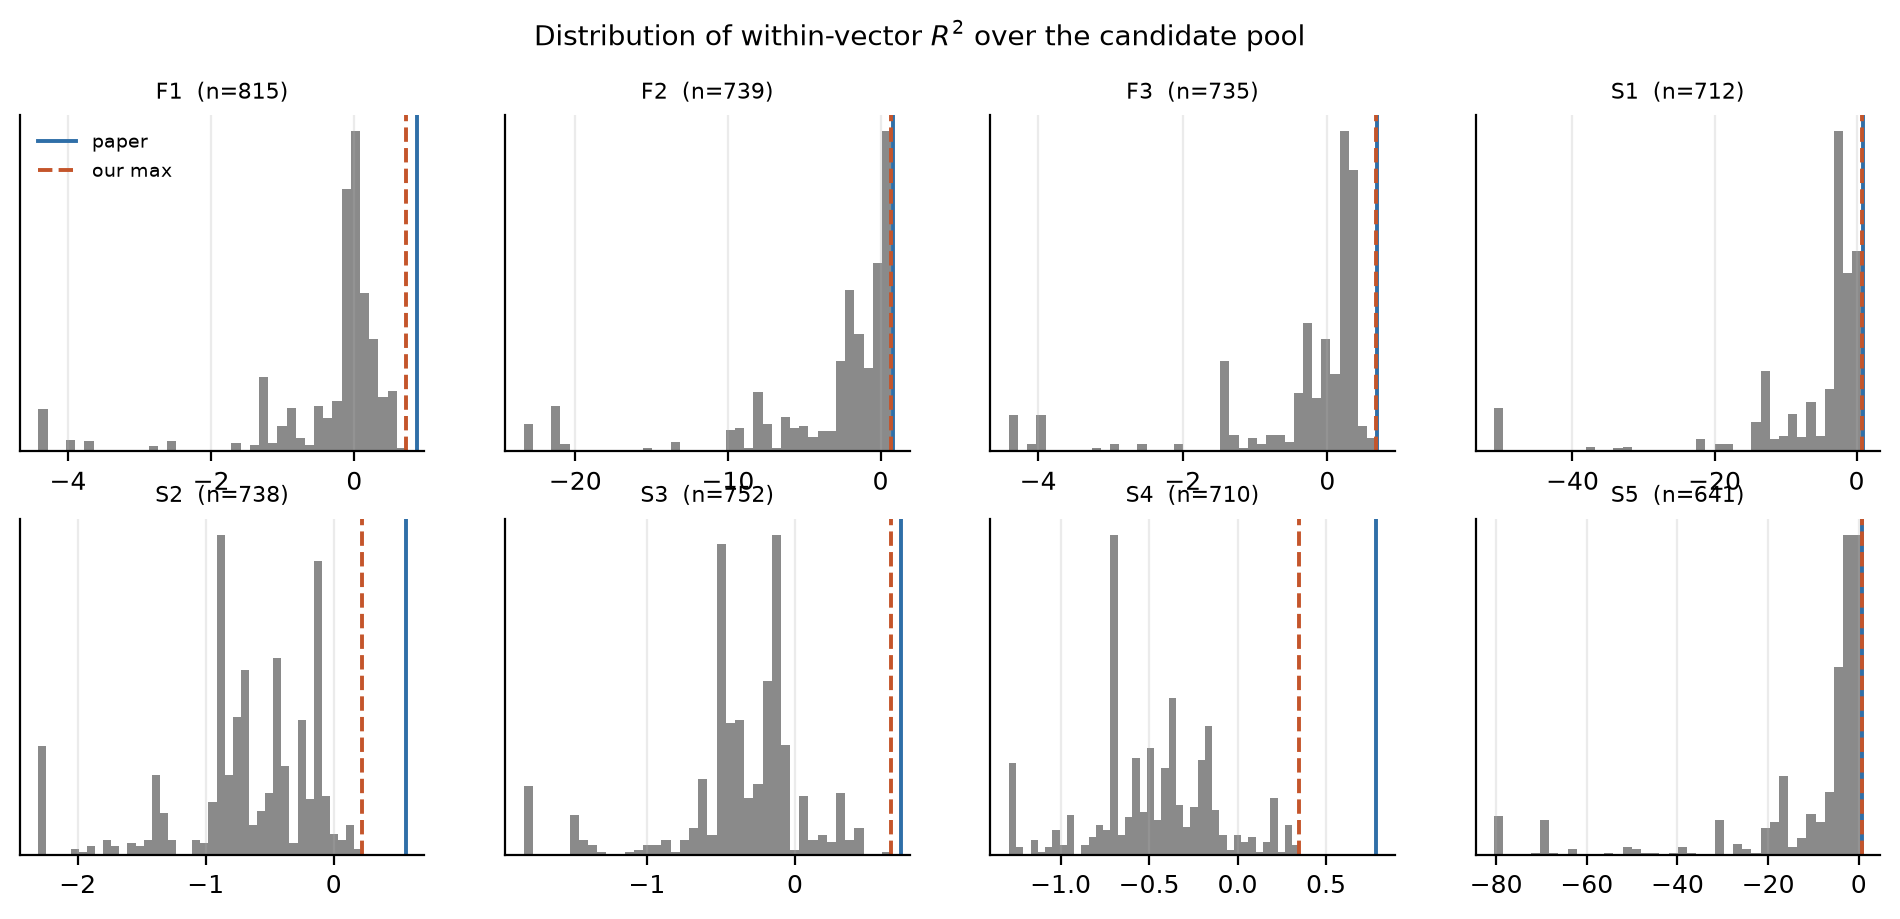
\includegraphics[width=\linewidth]{figures/fig3_r2_distribution.png}
\caption[R-squared distributions]{\textbf{The distribution the paper reports the
maximum of.} One panel per target; each histogram is the \Rsq{} of $\sim$700--800
individually generated candidates. The blue line is the paper's published
value, the dashed orange line is my pool maximum. Two things to see. First, the
mass of the distribution sits at or below zero --- the typical candidate is
worse than guessing the mean. Second, both vertical lines are far out in the
right tail, which is the visual statement of the whole best-of-$N$ argument.
The left tails are clipped at the 2nd percentile; they run to $-100$ and beyond
for some sets, which is why the means in Table~\ref{tab:repro} look extreme.}
\label{fig:r2dist}
\end{figure}

Bootstrapping from each pool gives the expected best score as a function of the
budget:

\begin{table}[htbp]
\centering\small
\caption[Best-of-N curves]{Expected best \Rsq{} after $N$ draws. Capped at
$N \le$ pool$/10$; beyond that the bootstrap is really just reporting the pool
maximum back, not estimating anything independent of it.}
\label{tab:bestofn}
\begin{tabular}{lccccccc}
\toprule
\textbf{set} & $N{=}1$ & $2$ & $4$ & $8$ & $16$ & $32$ & $64$ \\
\midrule
F1 & $-0.36$ & $+0.06$ & 0.23 & 0.34 & 0.44 & 0.51 & 0.56 \\
F2 & $-3.40$ & $-0.86$ & 0.05 & 0.40 & 0.54 & 0.58 & 0.59 \\
F3 & $-0.34$ & $+0.13$ & 0.30 & 0.37 & 0.42 & 0.47 & 0.54 \\
S1 & $-6.49$ & $-2.09$ & $-0.66$ & $-0.07$ & 0.26 & 0.44 & 0.55 \\
S2 & $-0.70$ & $-0.38$ & $-0.22$ & $-0.09$ & $-0.02$ & 0.03 & 0.09 \\
S3 & $-0.36$ & $-0.15$ & $+0.01$ & 0.12 & 0.25 & 0.35 & 0.42 \\
S4 & $-0.48$ & $-0.28$ & $-0.10$ & $+0.01$ & 0.14 & 0.23 & 0.28 \\
S5 & $-11.71$ & $-3.43$ & $-1.29$ & $-0.45$ & $-0.03$ & 0.21 & 0.34 \\
\bottomrule
\end{tabular}
\end{table}

\begin{figure}[htbp]
\centering

\includegraphics[width=0.92\linewidth]{figures/fig2_bestofn.png}
\caption[Best-of-N curves plotted]{\textbf{The same data as a curve.} Horizontal
axis is the sampling budget on a log scale; vertical axis is the expected best
\Rsq. Each colour is one target; dotted horizontal lines are the paper's
published values; shaded bands are 5th--95th percentiles over bootstrap
replicates. Every curve climbs steeply and monotonically. Nothing about the
model changes along these curves --- only how many times you ask it. The axis is
clipped at $-2$ because three sets have $N{=}1$ means below that.}
\label{fig:bestofn}
\end{figure}

\begin{goodbox}{Result}
A single draw from the inverse task is typically worse than useless: the median
candidate has negative \Rsq{} in six of eight sets. Essentially all of the
apparent performance is produced by generating many candidates and keeping the
best.
\end{goodbox}

\begin{keybox}{What does \emph{not} follow}
This is not a criticism of the method. Screening thousands of cheap candidates
is exactly the right procedure when generation costs nothing and evaluation
costs less. If you can make 2{,}000 designs and test them in silico, take the
best one --- obviously.

The objection is narrower, and it is about reporting. Given only the maximum, a
reader cannot tell how much search produced it, cannot compare it against
another method's single-shot number, and cannot estimate the compute needed to
match it. Stating $N$, or showing this curve, costs nothing and removes the
ambiguity entirely.
\end{keybox}

\section{Extension 2: what does the model read from the sequence?}
\label{sec:ablations}

If the forward task computes properties from sequence features, then editing
those features should move the prediction in interpretable ways. This
experiment does controlled surgery on 30 real MaSp sequences and measures how
far the prediction moves.

\subsection{Getting the reference points right}

Two things had to be established before any effect could be interpreted.

\paragraph{A floor.} How much does the prediction move when nothing
meaningful changes? The obvious answer --- resubmit the identical prompt --- gives
exactly zero under greedy decoding, by construction. That floor can never
reject anything, so it is useless as a safeguard. I therefore added a real one:
a \term{conservative point mutation}, one residue swapped for a chemically
similar one, the smallest edit that changes the sequence at all. Measured at
\textbf{0.0148}, with a median of exactly zero --- most single substitutions
change nothing.

\paragraph{A scale.} A shift of ``0.13'' means nothing without knowing the
range. Across 30 unmodified natural sequences, the model's output varies by
\textbf{0.0874}. Every effect below is quoted as a multiple of that.

\subsection{The edits}

\begin{figure}[htbp]
\centering
\begin{tikzpicture}[font=\scriptsize,
  seq/.style={draw=greyc!60,minimum height=0.45cm,inner sep=2pt},
  pa/.style={seq,fill=papercol!30},
  gg/.style={seq,fill=ourscol!25},
  o/.style={seq,fill=boxbg},
  lbl/.style={font=\scriptsize\bfseries,anchor=east},
]
% original
\node[lbl] at (-0.25,0) {original};
\node[o,minimum width=1.0cm] (a1) at (0.5,0) {};
\node[pa,minimum width=0.8cm,right=0pt of a1] (a2) {A$_n$};
\node[gg,minimum width=1.0cm,right=0pt of a2] (a3) {GGX};
\node[o,minimum width=0.9cm,right=0pt of a3] (a4) {};
\node[pa,minimum width=0.8cm,right=0pt of a4] (a5) {A$_n$};
\node[o,minimum width=1.1cm,right=0pt of a5] (a6) {};

% shuffle
\node[lbl] at (-0.25,-0.75) {shuffle};
\node[o,minimum width=5.6cm] at (3.3,-0.75) {same letters, order destroyed};

% knockout
\node[lbl] at (-0.25,-1.5) {knockout poly-A};
\node[o,minimum width=1.0cm] (c1) at (0.5,-1.5) {};
\node[gg,minimum width=1.0cm,right=0pt of c1] (c3) {GGX};
\node[o,minimum width=0.9cm,right=0pt of c3] (c4) {};
\node[o,minimum width=1.1cm,right=0pt of c4] (c6) {};
\node[right=0.2cm of c6,text=ourscol] {$\leftarrow$ poly-A blocks excised};

% scattered control
\node[lbl] at (-0.25,-2.25) {scattered control};
\node[o,minimum width=4.0cm] at (2.5,-2.25) {same \emph{number} of residues removed, at random positions};

% block control
\node[lbl] at (-0.25,-3.0) {block control};
\node[o,minimum width=4.0cm] at (2.5,-3.0) {same number removed, as \emph{one} contiguous run};
\end{tikzpicture}
\caption[Ablation design]{The ablation design. Each knockout is run against
\emph{two} length-matched controls, because removing residues changes two
things at once: which residues were removed, and how the removal was
distributed. Comparing against only one control confounds them.}
\label{fig:ablationdesign}
\end{figure}

\begin{figure}[htbp]
\centering

\includegraphics[width=0.94\linewidth]{figures/fig4_ablation.png}
\caption[Ablation results]{\textbf{How far each edit moves the prediction.}
Horizontal axis is the mean absolute change across the eight predicted values.
Grey bars are the length-matched controls; orange are the ablations of
interest. The dotted blue line at 0.087 is the spread the model shows across
genuinely different natural sequences --- a bar reaching it means the edit moved
the prediction as far as swapping in a different real spidroin would. The
bottom bar, \code{point\_mutation} at 0.015, is the floor.}
\label{fig:ablation}
\end{figure}

\subsection{Finding (a): no motif-specific effect}

\begin{table}[htbp]
\centering\small
\caption[Knockouts vs controls]{Every knockout lands \emph{between} its two
controls.}
\begin{tabular}{lccc}
\toprule
\textbf{motif} & \textbf{knockout} & \textbf{scattered control} & \textbf{block control} \\
\midrule
poly-A & 0.0809 & 0.1043 & 0.0493 \\
GGX & 0.0715 & 0.0914 & 0.0551 \\
GPGXX & 0.0954 & 0.1063 & 0.0429 \\
\bottomrule
\end{tabular}
\end{table}

A motif knockout removes several contiguous runs. Sitting between ``one block''
and ``scattered'' is precisely what removing that many residues \emph{without}
any motif-specific sensitivity predicts.

\begin{goodbox}{Result}
Removing poly-alanine tracts --- the $\beta$-sheet nanocrystal formers, the most
mechanically consequential motif in spider silk --- perturbs the prediction
\emph{less} than deleting the same number of residues at random positions. I
find no evidence that the forward task treats these motifs as special.
\end{goodbox}

\begin{warnbox}{The second control was essential}
Against the scattered control alone, poly-A knockout looks like a large effect
in the \emph{wrong} direction, which would have been a striking and wrong
finding. The block control shows it is not an effect at all --- only a difference
in how the deletion was distributed. I added that control after seeing the
first result look too interesting.
\end{warnbox}

\subsection{Finding (b): the output saturates}

Reversing the sequence (0.1322), shuffling it (0.1467), block-shuffling it
(0.1301) and replacing it with \emph{uniform random residues} (0.1230) all move
the prediction by about the same amount --- 1.4--1.7 times the spread across real
sequences. Past a certain amount of disruption, more disruption does not move
the output further.

\begin{warnbox}{Interpretation limits}
A shuffled spidroin is far outside the fine-tuning distribution. A large shift
shows the model is \emph{sensitive} to order without showing that it \emph{uses}
order meaningfully --- it may simply be reacting to text that does not look like
its training data. These measure the model, not spider silk, and no claim about
real mechanical behaviour follows.
\end{warnbox}

\section{Extension 3: how far do amino-acid counts alone get you?}
\label{sec:baseline}

A control. If a ridge regression on letter frequencies does as well as a
253-million-parameter transformer, that reframes what the transformer
contributes.

\begin{figure}[htbp]
\centering
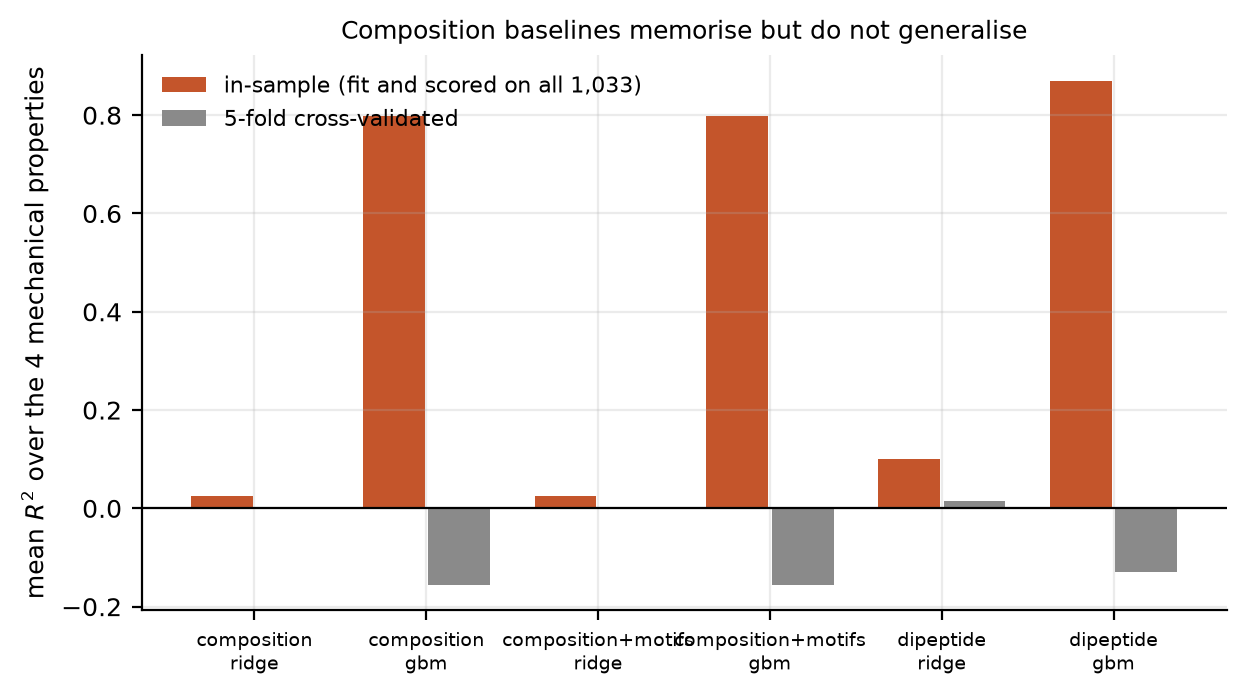
\includegraphics[width=0.88\linewidth]{figures/fig5_baseline.png}
\caption[Baseline]{\textbf{Composition baselines memorise but do not
generalise.} Each pair of bars is one feature set and model. Orange is
in-sample (fit and scored on all 1{,}033 rows); grey is 5-fold
cross-validated. Gradient boosting reaches $R^2 \approx 0.80$--$0.87$ in-sample
and \emph{negative} under cross-validation --- worse than predicting the dataset
mean. The gap between the two bars is the entire point of the figure.}
\label{fig:baseline}
\end{figure}

\begin{table}[htbp]
\centering\small
\caption[Baseline numbers]{Mean \Rsq{} over the four mechanical properties.}
\begin{tabular}{llcc}
\toprule
\textbf{features} & \textbf{model} & \textbf{in-sample} & \textbf{5-fold CV} \\
\midrule
composition & ridge & 0.026 & 0.001 \\
composition & GBM & \textbf{0.799} & \textbf{$-0.155$} \\
composition + motifs & ridge & 0.025 & 0.004 \\
composition + motifs & GBM & 0.798 & $-0.155$ \\
dipeptide & ridge & 0.100 & 0.014 \\
dipeptide & GBM & 0.870 & $-0.130$ \\
\bottomrule
\end{tabular}
\end{table}

Species-grouped cross-validation, where no species appears in both training and
test folds, gives $-0.049$.

\begin{goodbox}{Result}
On this dataset, in-sample fit and generalisation are close to \emph{unrelated}.
A model can reach 0.87 in-sample while being worse than useless out of sample.
Since the paper fine-tunes on all 1{,}033 pairs and holds nothing out, that
warning applies to any forward-task accuracy measured on them --- the paper's
and mine alike.
\end{goodbox}

\subsection{The baseline on Table 1's own axis}

Scoring the same baseline the paper's way --- within-vector \Rsq, one value per
sequence --- puts it on the only axis directly comparable to the headline
numbers:

\begin{center}
\small
\begin{tabular}{lc}
\toprule
composition ridge on real pairs & mean $-1.70$, median $-0.22$, \textbf{max 0.697} \\
paper, eight targets & 0.564 -- 0.890 \\
this project, eight targets & 0.223 -- 0.722 \\
\bottomrule
\end{tabular}
\end{center}

\begin{warnbox}{Not a like-for-like comparison}
The baseline figure is the maximum over 1{,}033 \emph{in-sample fits} to
sequences whose labels it trained on. The paper's is the maximum over $\sim$2{,}000
\emph{generated} sequences scored against a target never in any training set.
Different procedures, different denominators.

What the number does show is that a value in the 0.6--0.7 band \emph{on this
metric} is reachable without a transformer and without generation --- worth
knowing before reading any single such value as evidence of sequence
understanding.
\end{warnbox}

\section{Extension 4: what happens outside MaSp?}
\label{sec:nonmasp}

The model is fine-tuned on MaSp only. The database contains seven other
spidroin families from the same individuals. The forward task accepts them
without complaint.

\begin{figure}[htbp]
\centering
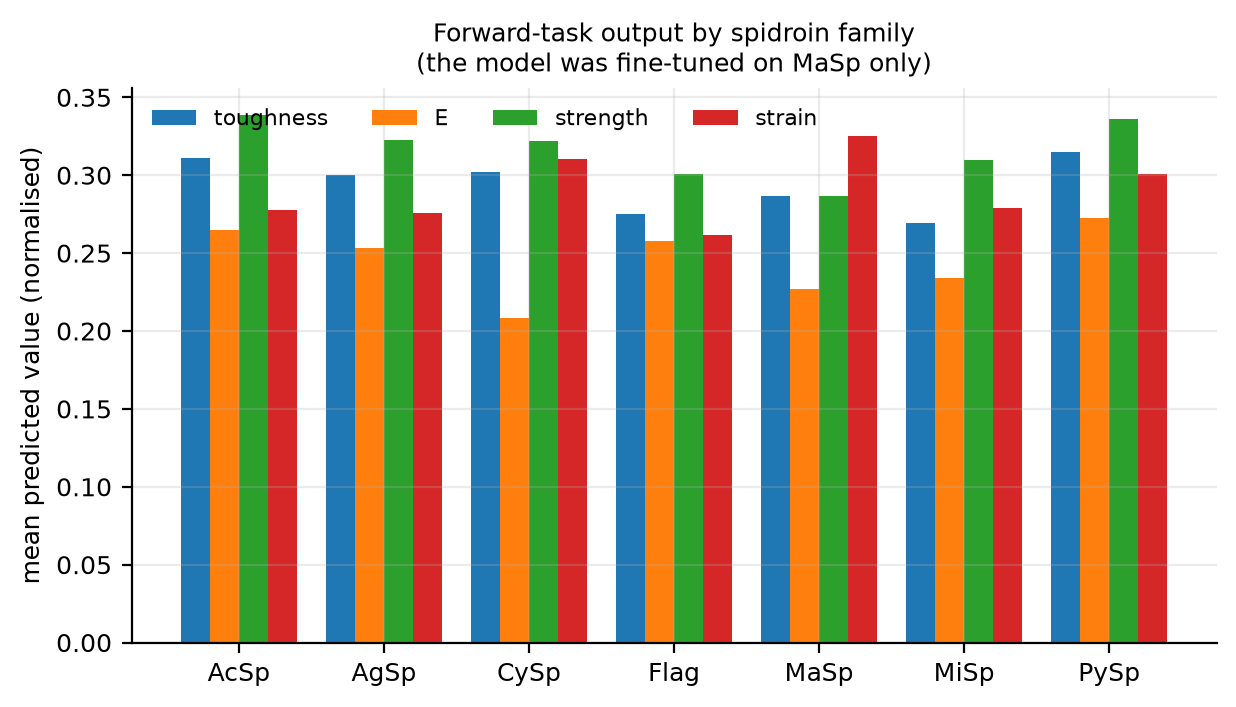
\includegraphics[width=0.88\linewidth]{figures/fig6_nonmasp.png}
\caption[Non-MaSp predictions]{\textbf{Mean prediction by spidroin family.}
Four bars per family, one per mechanical property. If the model were reading
the sequence deeply, families as different as Flag (the stretchy capture
spiral) and MaSp (the stiff dragline) should look different. They barely do ---
every family's bars sit at nearly the same heights.}
\label{fig:nonmasp}
\end{figure}

\begin{table}[htbp]
\centering\small
\caption[Accuracy by family]{Accuracy against measured dragline properties.}
\begin{tabular}{lccc}
\toprule
\textbf{family} & \textbf{in training?} & \textbf{mean \Rsq} & \textbf{mean abs.\ error} \\
\midrule
MaSp & \textbf{yes} & \textbf{$+0.826$} & 0.024 \\
MiSp & no & $-0.270$ & 0.141 \\
AcSp & no & $-0.317$ & 0.170 \\
AgSp & no & $-0.430$ & 0.158 \\
CySp & no & $-0.472$ & 0.151 \\
Flag & no & $-0.514$ & 0.161 \\
PySp & no & $-0.540$ & 0.152 \\
\bottomrule
\end{tabular}
\end{table}

Accuracy falls off a cliff outside MaSp, from $+0.83$ to between $-0.27$ and
$-0.54$, with error rising six-fold.

And the predictions barely depend on family at all. The between-family spread of
the mean prediction is \textbf{0.019} against a within-family spread of
\textbf{0.095} --- a ratio of \textbf{0.199}, both measured over the same four
mechanical properties.

\begin{goodbox}{Result}
Handed a spidroin it has not memorised, the model emits something close to its
training marginal regardless of which silk family the sequence came from.
\end{goodbox}

\begin{warnbox}{The caveat, stated before the numbers are used}
Silkome's mechanical properties are measured on \emph{dragline}, which is MaSp.
A Flag sequence here is paired with the same spider's dragline properties, not
with flagelliform properties. So this is \emph{not} a test of whether the model
can predict flagelliform silk --- no analysis of this dataset could be. It is
the narrower question of whether a non-MaSp sequence from an individual still
recovers that individual's dragline properties.

The between/within ratio needs no such caveat: it uses no ground truth at all.
\end{warnbox}

\section{The thing all four extensions point at}
\label{sec:memorisation}

Four independent measurements converge.

\subsection{The forward task returns training labels verbatim}

Over the 1{,}033 fine-tuning pairs, the forward task's in-sample \Rsq{} averages
0.696 across the four mechanical properties. Respectable. But:

\begin{goodbox}{732 of 1{,}026 scored rows --- 71.3\% --- come back with all eight
values \emph{identical} to the training label}
to within 0.0005, which is the resolution the model can express. Mean absolute
error on those rows is 0.00025. On the remaining 294 rows it is 0.109, and the
mean \Rsq{} is $\mathbf{-0.113}$: worse than predicting the dataset mean.
\end{goodbox}

\begin{figure}[htbp]
\centering
\begin{tikzpicture}[font=\small]
\begin{axis}[
  width=12cm,height=4.4cm,
  xbar stacked, xmin=0, xmax=1026,
  ytick=\empty, y=1.1cm,
  xlabel={fine-tuning pairs}, xlabel style={font=\scriptsize},
  bar width=0.7cm, axis lines=left,
  legend style={font=\scriptsize,draw=none,at={(0.5,-0.42)},anchor=north,legend columns=2},
  clip=false,
]
\addplot[fill=ourscol!35,draw=ourscol] coordinates {(732,0)};
\addlegendentry{label returned exactly (71.3\%), error 0.00025}
\addplot[fill=greyc!25,draw=greyc] coordinates {(294,0)};
\addlegendentry{everything else, mean $R^2 = -0.113$}
\end{axis}
\end{tikzpicture}
\caption[Memorisation]{The composition of the in-sample \Rsq{} of 0.696. Most
of it rests on rows where the model returned the training label verbatim rather
than predicting anything.}
\label{fig:memorisation}
\end{figure}

\subsection{The inverse task returns training sequences verbatim}
\label{sec:regurgitation}

\begin{center}
\small
\begin{tabular}{lccc}
\toprule
\textbf{set} & \textbf{parsed} & \textbf{verbatim copies} & \textbf{copy rate} \\
\midrule
F1 & 1946 & 1122 & 57.7\% \\
F2 & 1961 & 1219 & 62.2\% \\
F3 & 1949 & 1208 & 62.0\% \\
S1 & 1953 & 1237 & 63.3\% \\
S2 & 1948 & 1206 & 61.9\% \\
S3 & 1955 & 1194 & 61.1\% \\
S4 & 1958 & 1243 & 63.5\% \\
S5 & 1974 & 1324 & 67.1\% \\
\midrule
\textbf{overall} & & & \textbf{62.3\%} \\
\bottomrule
\end{tabular}
\end{center}

Nearly two thirds of generations are byte-identical to sequences in the
reference set. These are not a handful of repeats --- 200 to 290 \emph{distinct}
known sequences appear per set. A nominal budget of 2{,}048 therefore yields
about 771 scoreable candidates.

This contradicts nothing in the paper, which analyses only the novel outputs.
But the discard rate is not reported, and it means the model's default
behaviour in the inverse direction includes a great deal of retrieval.

\subsection{Putting it together}

\begin{keybox}{The picture}
\begin{itemize}[leftmargin=*,itemsep=2pt]
  \item Forward: returns the exact training label 71\% of the time; on the rest,
        worse than the mean.
  \item Inverse: returns a verbatim training sequence 62\% of the time.
  \item Outside its training family: accuracy collapses, $+0.83 \to -0.27\ldots-0.54$.
  \item Its output barely varies with family: ratio 0.199.
  \item A composition baseline shows the underlying task is genuinely hard ---
        cross-validated \Rsq{} near zero.
\end{itemize}
The pipeline behaves substantially like a \emph{retrieval system} over its
fine-tuning set, in both directions.
\end{keybox}

\begin{warnbox}{Three qualifications, because this invites overreading}
\textbf{It contradicts nothing the paper claims.} The paper fine-tunes on all
pairs, says so, reports self-consistency rather than held-out accuracy, and
makes no generalisation claim. Memorisation is the \emph{expected} consequence
of training on everything and evaluating on the same data.

\textbf{The $-0.113$ is not a generalisation estimate.} Those rows are selected
on the outcome, and they differ systematically from the rest --- median length
456 against 361. Selecting on the outcome biases the estimate downward by an
unknown amount. A real held-out number requires retraining with a fold held
out, which I did not do.

\textbf{The task is genuinely hard.} The composition baseline establishes that
nobody --- not the transformer, not ridge regression --- has demonstrated
generalisation on this dataset. That is a property of the problem, not of any
particular model.
\end{warnbox}

\section{The reproduction of Table 1, seen whole}

\begin{figure}[htbp]
\centering
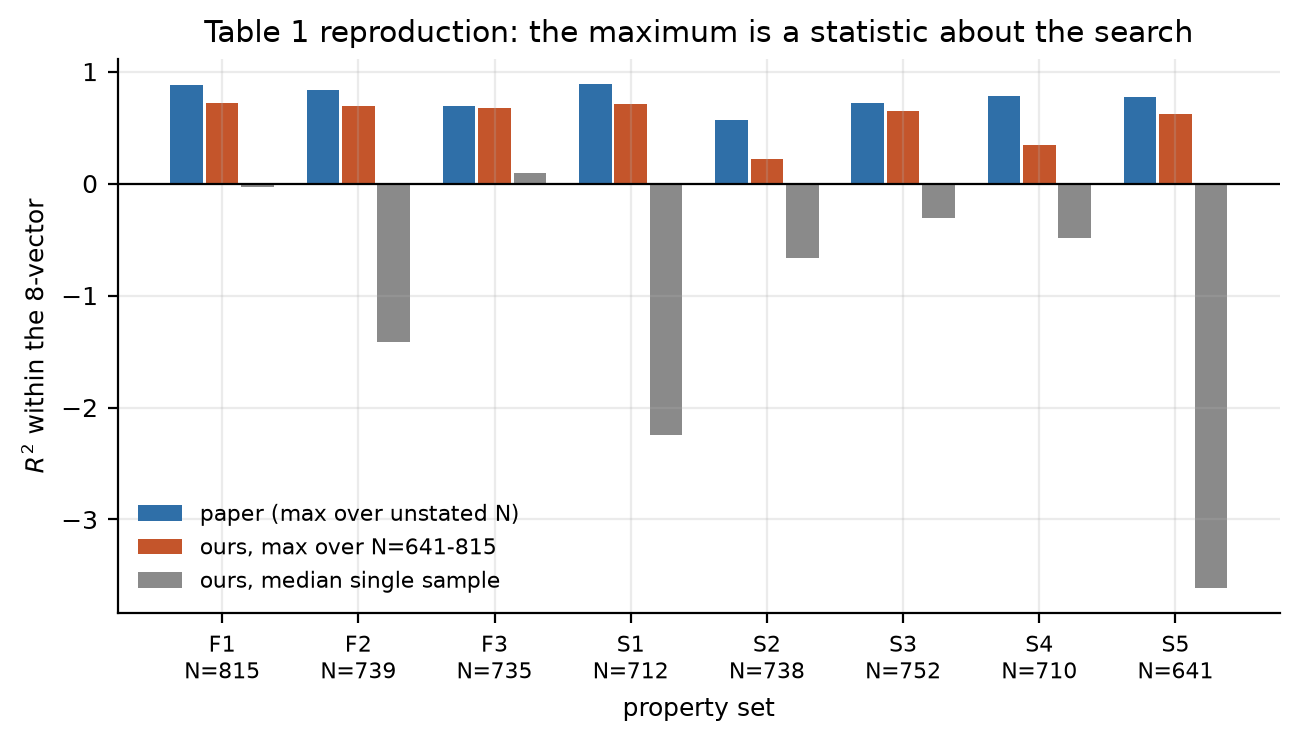
\includegraphics[width=\linewidth]{figures/fig1_table1_reproduction.png}
\caption[Table 1 reproduction]{\textbf{The headline comparison.} For each
target: blue is the paper's published \Rsq{} (a maximum over an unstated $N$),
orange is my pool maximum, grey is my \emph{median} single candidate. The tick
labels give each set's scoreable pool size. The orange bars fall short
everywhere --- that is the shortfall of Section~\ref{sec:table1}, now known to
live in the search rather than the model. The grey bars are the more
informative ones: they show what a single draw from this pipeline is typically
worth, and for six of eight targets that is below zero.}
\label{fig:table1}
\end{figure}
